\documentclass[italian, a4paper, 12pt]{article}

\usepackage[utf8]{inputenc}
\usepackage[T1]{fontenc}
\usepackage{babel}

\usepackage[left=25mm, top=20mm, right=25mm, bottom=20mm]{geometry}
\renewcommand{\baselinestretch}{1.5}

\usepackage{float}

%%% font & looks %%%
\usepackage{mathpazo}
%\usepackage{palatino}
%\usepackage{kpfonts}
%\usepackage{times}
%\usepackage{charter}
%\usepackage{utopia}

% list of fonts available here - http://www.tug.dk/FontCatalogue/
% and here - https://www.sharelatex.com/learn/Font_typefaces

\usepackage{microtype}

\usepackage[parfill]{parskip}

\usepackage{bm}
\usepackage[labelfont=bf,font={small,it}]{caption}
\usepackage[usenames,dvipsnames,svgnames,table]{xcolor}

\usepackage{newtxtext}
\usepackage{newtxmath}

%%% boxes %%%
\usepackage{framed}
%\setlength\FrameSep{0.5em}

% math
%\usepackage{amsmath}
\usepackage{amssymb}
%\usepackage{amsthm}
\usepackage{wasysym}
%\usepackage{siunitx}

% graphics
\usepackage{multirow}
\usepackage[section]{placeins}
\usepackage{graphicx}
\usepackage{epstopdf}
\usepackage{pgfplots}
  \pgfplotsset{compat=newest}
  %% the following commands are needed for some matlab2tikz features
  \usetikzlibrary{plotmarks}
  \usetikzlibrary{arrows.meta}
  \usepgfplotslibrary{patchplots}
  \usepackage{grffile}
  \usepackage{amsmath}

\usepackage{pdfpages}

% extra
\usepackage{todonotes} %\todo{ note } , \listoftodos
\usepackage{blindtext}
\usepackage{lipsum}
\usepackage{tikz}
\usetikzlibrary{patterns}
\usetikzlibrary{decorations.pathreplacing,angles,quotes}
\usepackage{chemformula}
\usepackage{textcomp}
\usepackage{subcaption}

% better tables
\usepackage{booktabs}

%%% links %%%
\usepackage{hyperref}
\hypersetup{
        linktocpage,
        colorlinks,
    citecolor=black,
    filecolor=black,
    linkcolor=black,
    urlcolor=black
}

\usepackage[framed,numbered]{matlab-prettifier}
\tikzset{
  font={\fontsize{9pt}{12}\selectfont}}

\usepackage[backend=biber]{biblatex}
\addbibresource{report.bib}

%%% references %%%
\usepackage[noabbrev,capitalize,nameinlink]{cleveref}

% new commands
\newcommand{\horline}{\rule{1\linewidth}{0.9pt}}
\newcommand{\curl}{\nabla \times}
\renewcommand{\div}{\nabla \cdot}
\newcommand{\laplac}{\nabla^2}
\newcommand{\grad}{\nabla}

%\usepackage{mathspec}

%\newcommand{\mathbbm}[1]{\text{\usefont{U}{bbm}{m}{n}#1}} % from mathbbm.sty
%\newcommand{\indi}[1]{\operatorname{\mathbbm{1}}\left[#1\right]}
\newcommand{\mathbbm}[1]{\text{\usefont{U}{bbm}{m}{n}#1}} % from mathbbm.sty


\newtheorem{p}{\\[5mm] \large Problem}
\newenvironment{s}{%\small%
        \begin{trivlist} \item \textbf{Solution}. }{%
\end{trivlist}}%
\begin{document}
\begin{center}
        %\horline\\
        \Large Wireless Systems And Networks\\
        \huge \textbf{Project: Unequal Error Protection}\\[3mm]
        \begin{framed}
                \Large \textbf{Workgroup} \\[2mm]
                \normalsize \textbf{Costa} Roberto -- \textbf{Zanol} Riccardo
        \end{framed}
        %\horline
\end{center}
\FloatBarrier
\section*{Sommario}
La tesina si prefigge di implementare un protocollo per trasmettere flussi video attraverso una rete non completamente affidabile, utilizzando un codice di correzione degli errori a fontana, il quale regola la ridondanza aggiunta ai dati in base alla loro importanza e in base alle necessità di ritrasmissione dei ricevitori.
Verrà analizzata la correttezza della trasmissione (in termini di Bit Error Rate e di PSNR) al variare della Bit Error Rate del canale. Verranno inoltre analizzate la complessità computazionale di codifica e decodifica e il tempo ad esse associato, al variare della ridondanza aggiunta.\\
Il progetto è stato realizzato in C++; Python è stato usato per riportare graficamente i risultati ottenuti.
\newpage
\section{Introduzione}
Spesso, al giorno d'oggi, la qualità delle connessioni tra i dispositivi di una rete è variabile, anche, ad esempio, a causa di meccanismi di condivisione di risorse adattativi, finalizzati al rispetto di vincoli variabili di throughput per un numero variabile di utenti. Variabile è anche l'insieme di dispositivi connessi alla rete e il link budget di ogni dispositivo. Quando è necessario trasmettere un flusso video a un insieme di utenti, la qualità del video, in questo tipo di rete, dev'essere necessariamente variabile in base alla banda disponibile ad ogni utente. Un protocollo che si presta al multicast video attraverso connessioni eterogenee è l'estensione Scalable Video Coding (SVC) del protocollo H.264/MPEG-4 AVC. Tale protocollo, infatti, permette di codificare il video una sola volta per tutti gli utenti, separando il file originale in un numero arbitrario di stream, la cui composizione garantisce alta fedeltà di ricostruzione del flusso video originale, ma non è indispensabile avere tutti le componenti per ricostruire il video a qualità arbitraria.\\
Più nel dettaglio, il flusso video codificato è organizzato in unità NAL (Network Abstraction Layer) che possono essere di 2 tipi: VCL NAL Packets (Video Coding Layer) e non-VCL NAL packets. I pacchetti non-VCL possono contenere il set di parametri da usare per decodificare (informazioni necessarie per la decodifica, quindi ad alta priorità), oppure delle informazioni supplemenari per migliorare la decodifica (SEI, Supplemental Enhancement Information). Il bitstream NAL è composto da una serie di sequenze video più corte (GOP, Group Of Pictures) decodificabili indipendentemente dal resto del flusso: ogni GOP comincia con tutte le informazioni necessarie alla decodifica, in modo che essa possa avvenire anche senza aver decodificato nessun segmento precedente.\\
Per trasmettere un flusso di dati attraverso un canale variabile e non completamente affidabile, garantendo la qualità del servizio, è utile aggiungere ridondanza all'informazione inviata. Il rapporto tra il messaggio con ridondanza aggiunta e il messaggio originale è chiamato rate del codice di correzione degli errori.
I codici a fontana presentano due caratteristiche notevoli, rispetto ad altri codici di correzione degli errori:
\begin{itemize}
\item Bassa complessità computazionale per la codifica e per la decodifica
\item Assenza di un code rate fisso.
\end{itemize}
I codici a fontana possono proteggere allo stesso modo tutti i dati da trasmettere, caso in cui la ridondanza aggiunta dipende solo dalle condizioni del canale (EEP, equal error protection), oppure possono proteggere maggiormente i dati più sensibili (UEP, unequal error protection), caso in cui la ridondanza aggiunta dipende anche dall'importanza del dato.\\
Un tipo di applicazione che si presta particolarmente all'utilizzo di UEP è lo streaming di un video codificato attraverso SVC, infatti tale protocollo rende possibile la decodifica di un flusso video da flussi parziali, chiamati \textit{layer}, con risoluzione spaziale o temporale minore, o con fedeltà ridotta. I layer sono ordinati dal più importante (layer 0, a bassa qualità) al meno importante (layer \textit{n}, che permette di raggiungere alta qualità).\\
La presenza di informazioni più rilevanti di altre (come i parametri per la decodifica, il primo pacchetto di ogni GOP o i layer inferiori) giustifica l'uso di UEP: i flussi con priorità minore aggiungono qualità al video decodificato, ma non sono indispensabili per la decodifica, quindi possono essere protetti con meno ridondanza.\\
Il vantaggio di aggiungere una quantità variabile di ridondanza, oltre che nel proteggere meglio i dati più sensibili, risiede anche nella possibilità di sfruttare un canale che ha un comportamento variabile nel tempo e ignoto a priori: la quantità di ridondanza aggiunta può crescere al peggiorare delle condizioni del canale, a differenza di un codice a rate fisso che comporta uno spreco di banda se il canale è in buone condizioni, o insufficiente protezione se il canale non è in buone condizioni.\\
Il canale considerato nelle simulazioni presenta errori i.i.d. con probabilità $e \in [10^{-8},10^{-1}]$.
\section{Approccio tecnico}
\subsection{Obbiettivi}
La finalità del progetto è testare l'algoritmo di trasmissione su un canale non privo di errori per dimostrare che.

\subsection{Diagramma}
%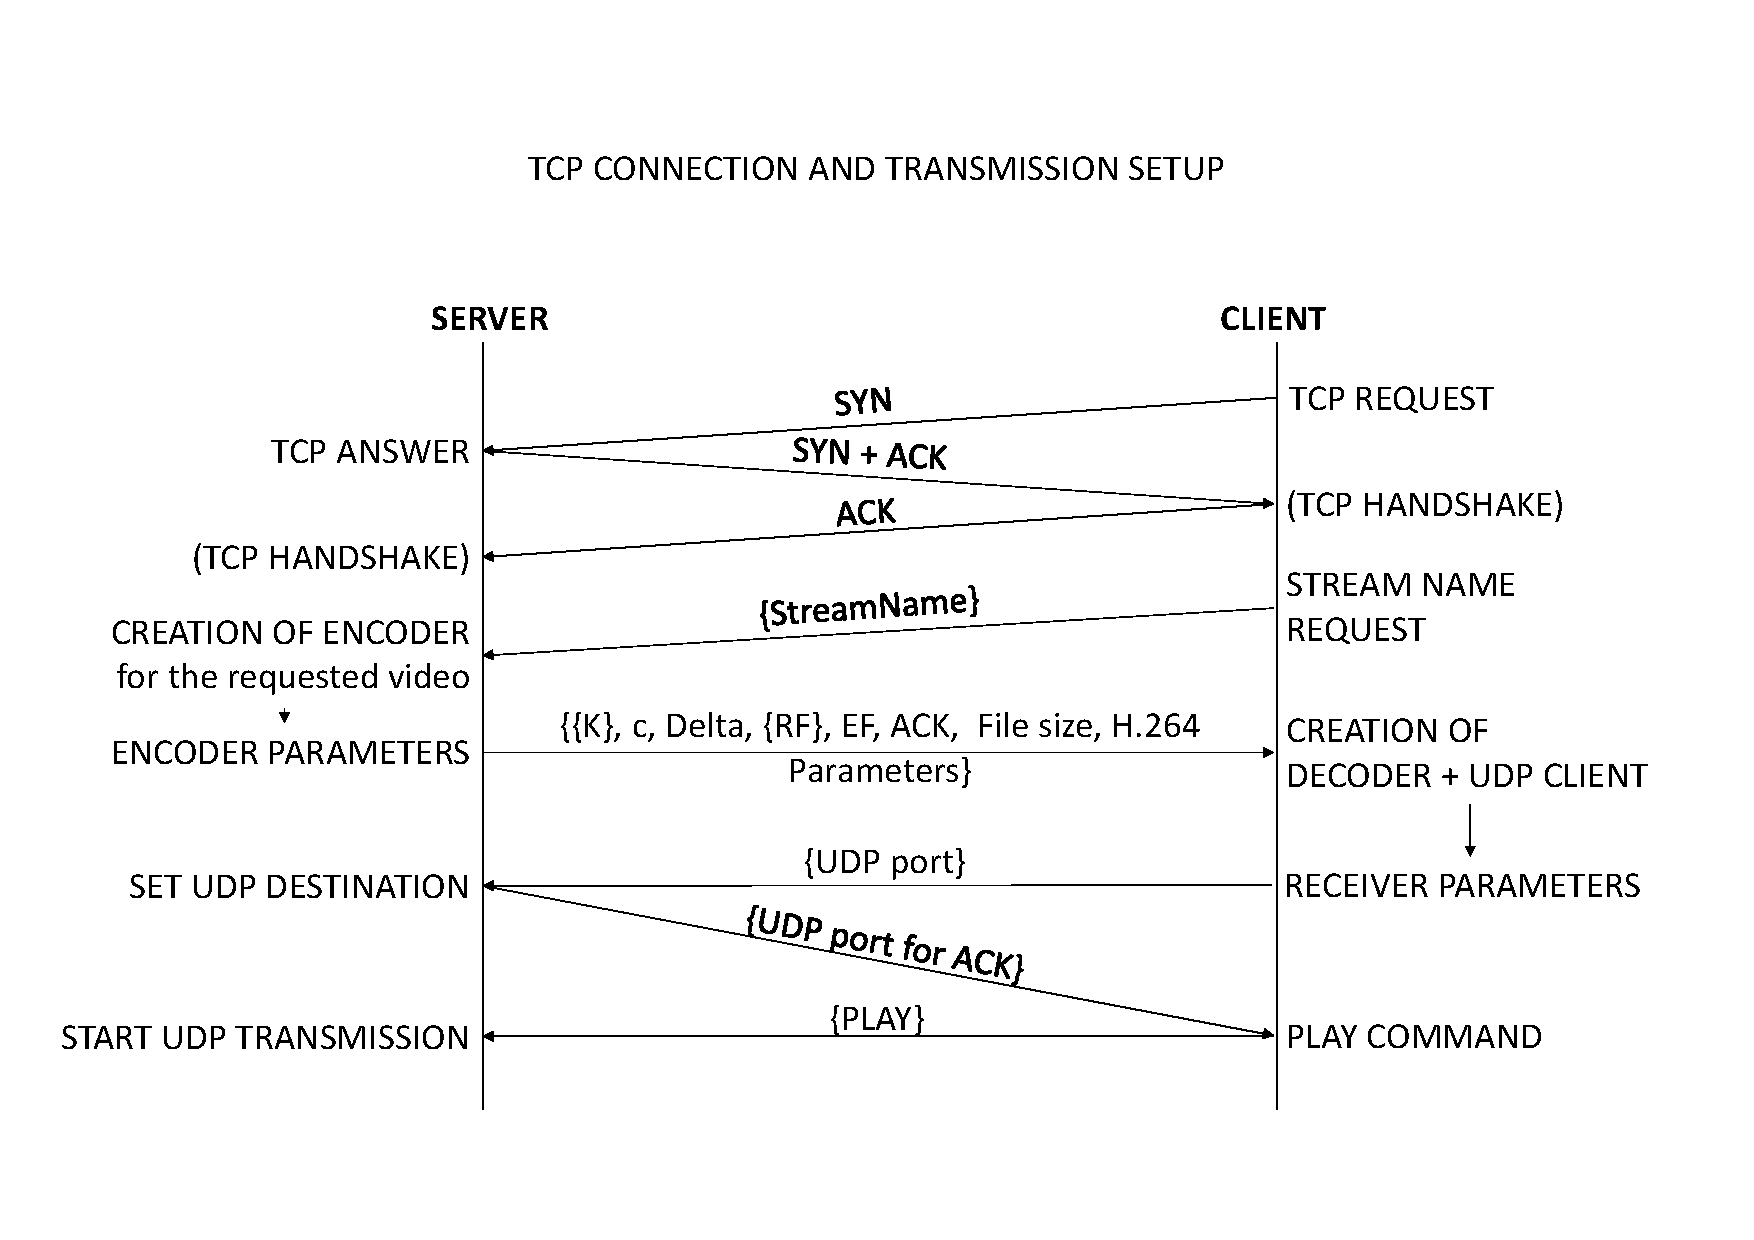
\includegraphics[trim=0cm 8cm 0cm 7cm, width=1.00\textwidth]{TCP.pdf}
%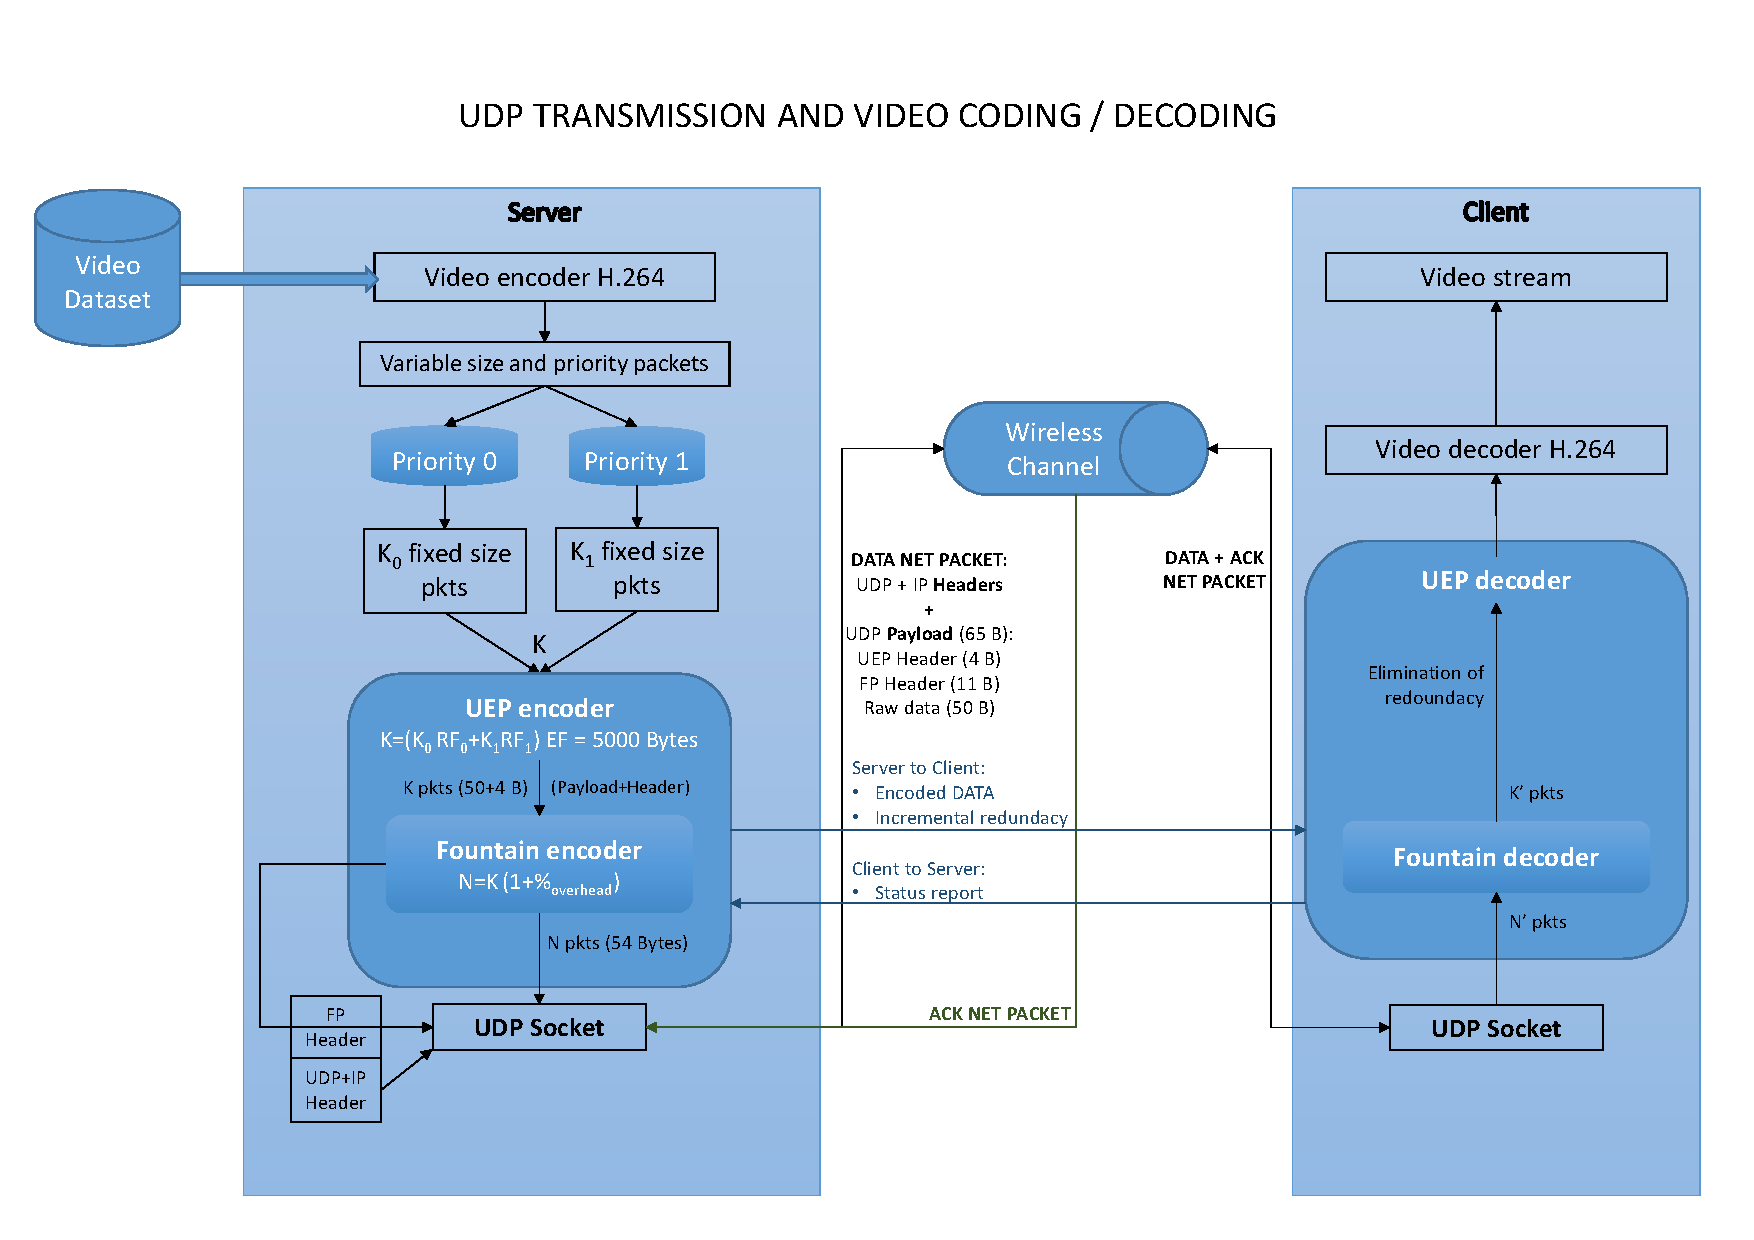
\includegraphics[width=180mm]{UDP.pdf}
%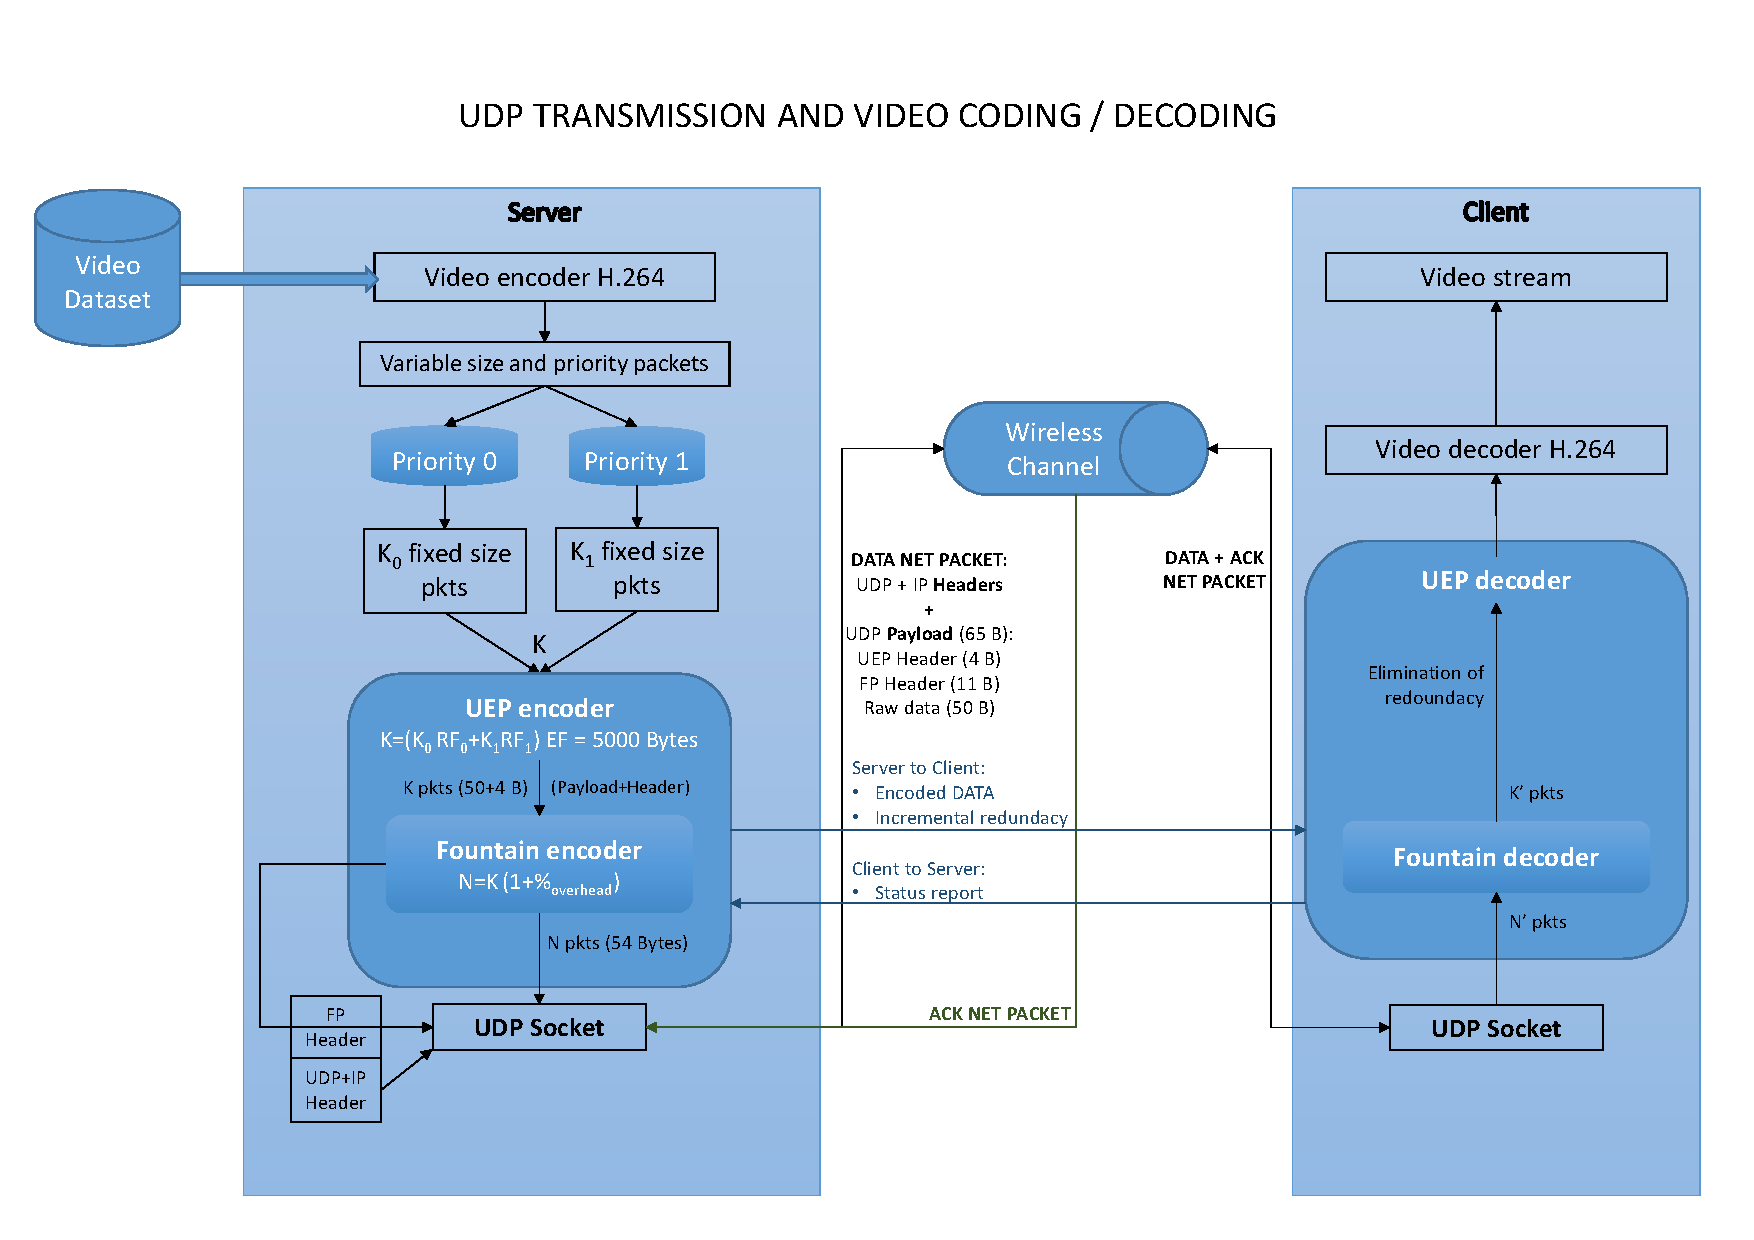
\includepdf[pages={1}]{UDP.pdf}
%\begin{figure}[htbp]
\begin{figure}[H]
    \centering
        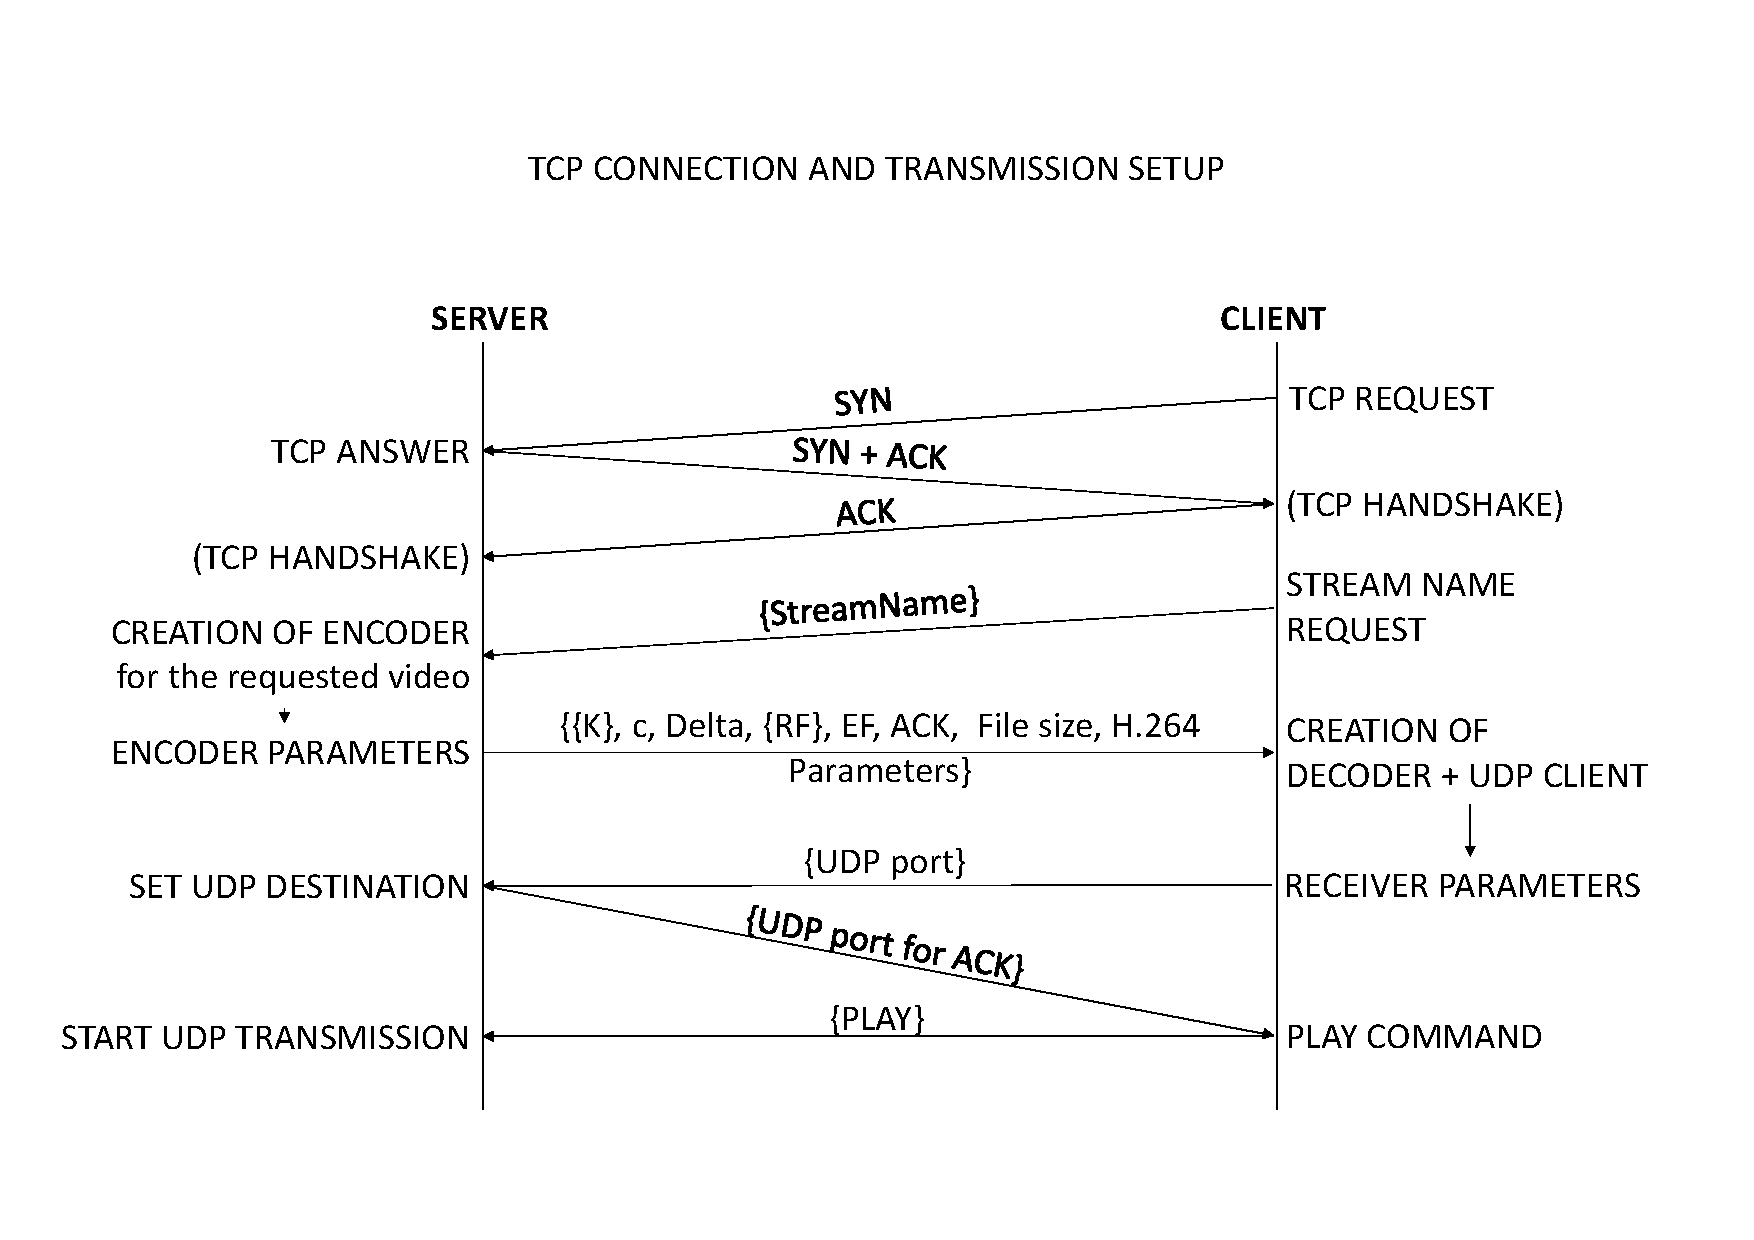
\includegraphics[clip, trim=0cm 1cm 0cm 1cm, width=1.00\textwidth]{TCP.pdf}
    \caption{TCP connection and tansmission setup}
    \label{fig:TCP}
\end{figure}
\begin{figure}[H]
    \centering
        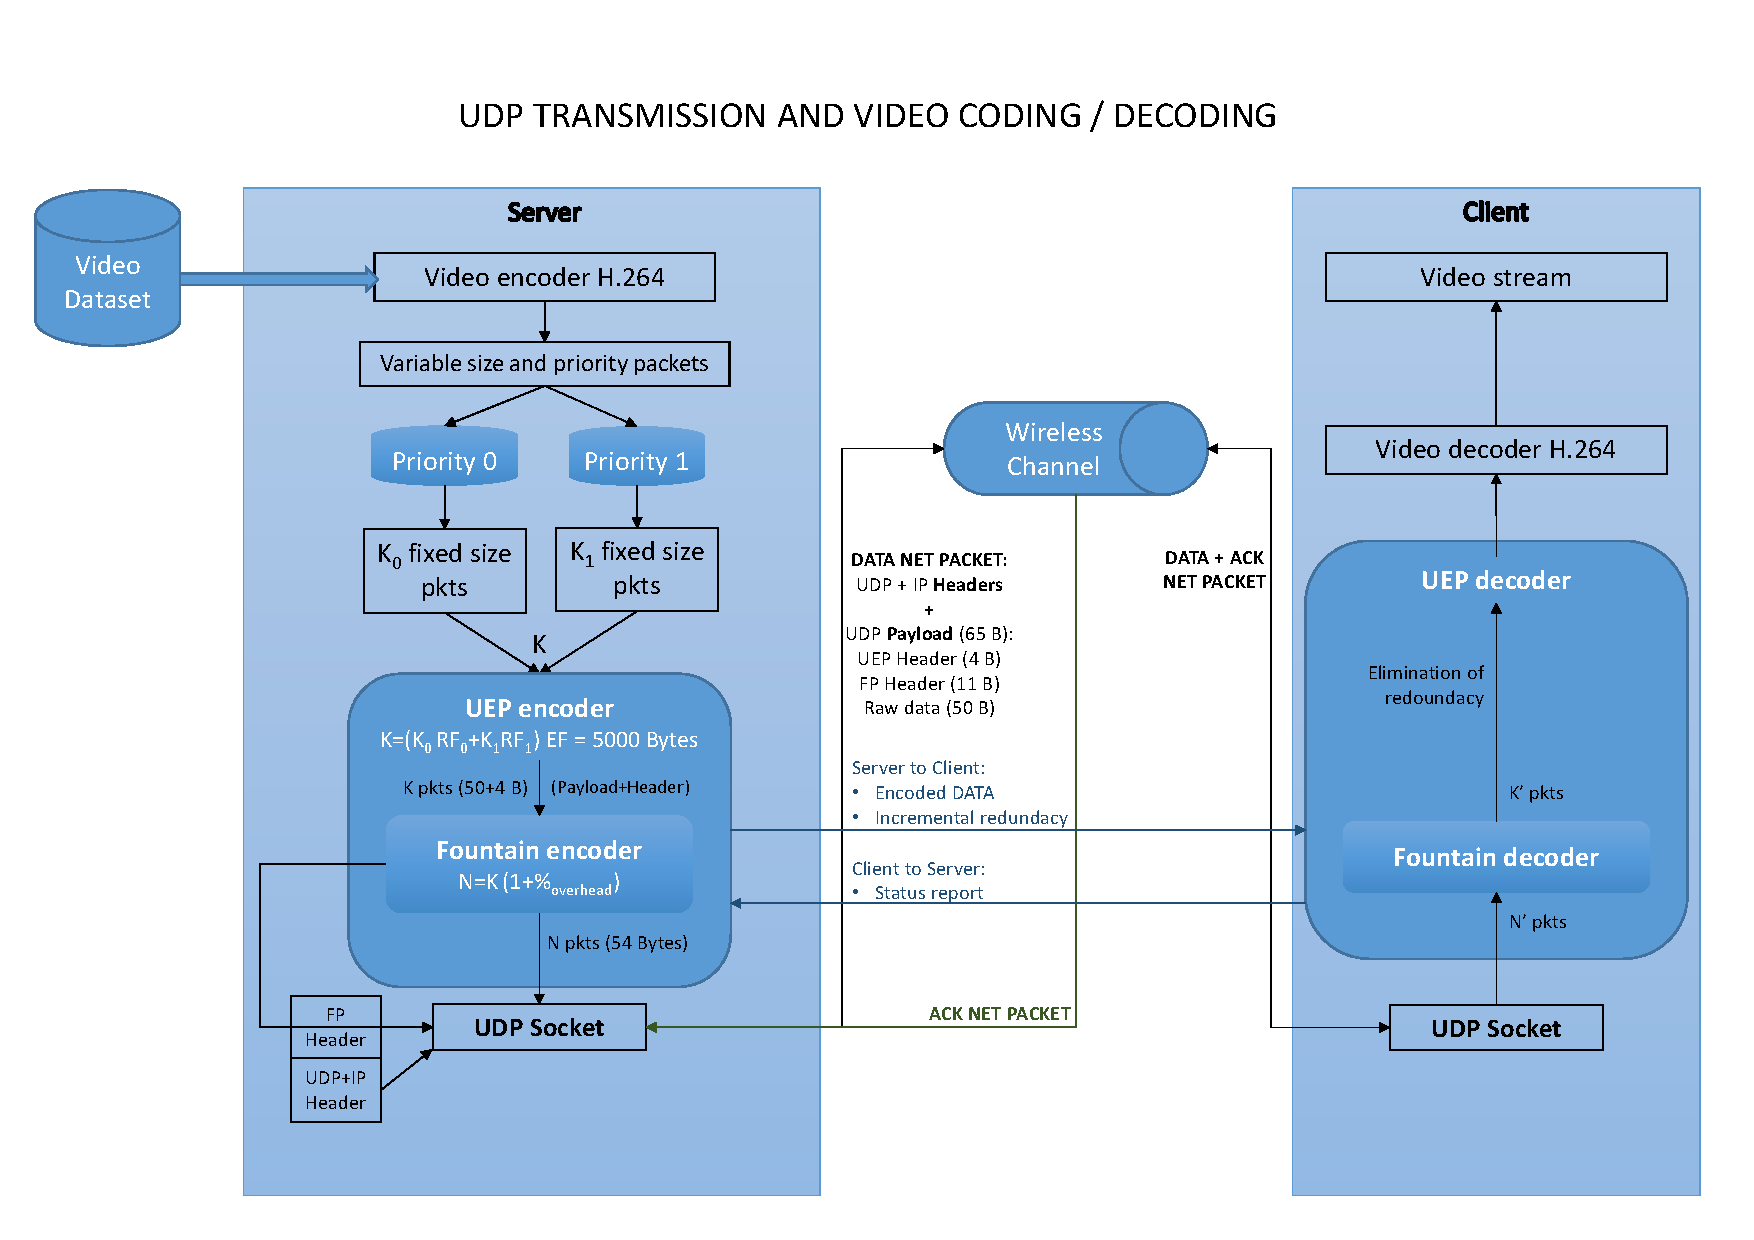
\includegraphics[clip, trim=0cm 1cm 0cm 1cm, width=1.00\textwidth]{UDP.pdf}
    \caption{Video stream encoding / decoding and transmission}
    \label{fig:UDP}
\end{figure}
%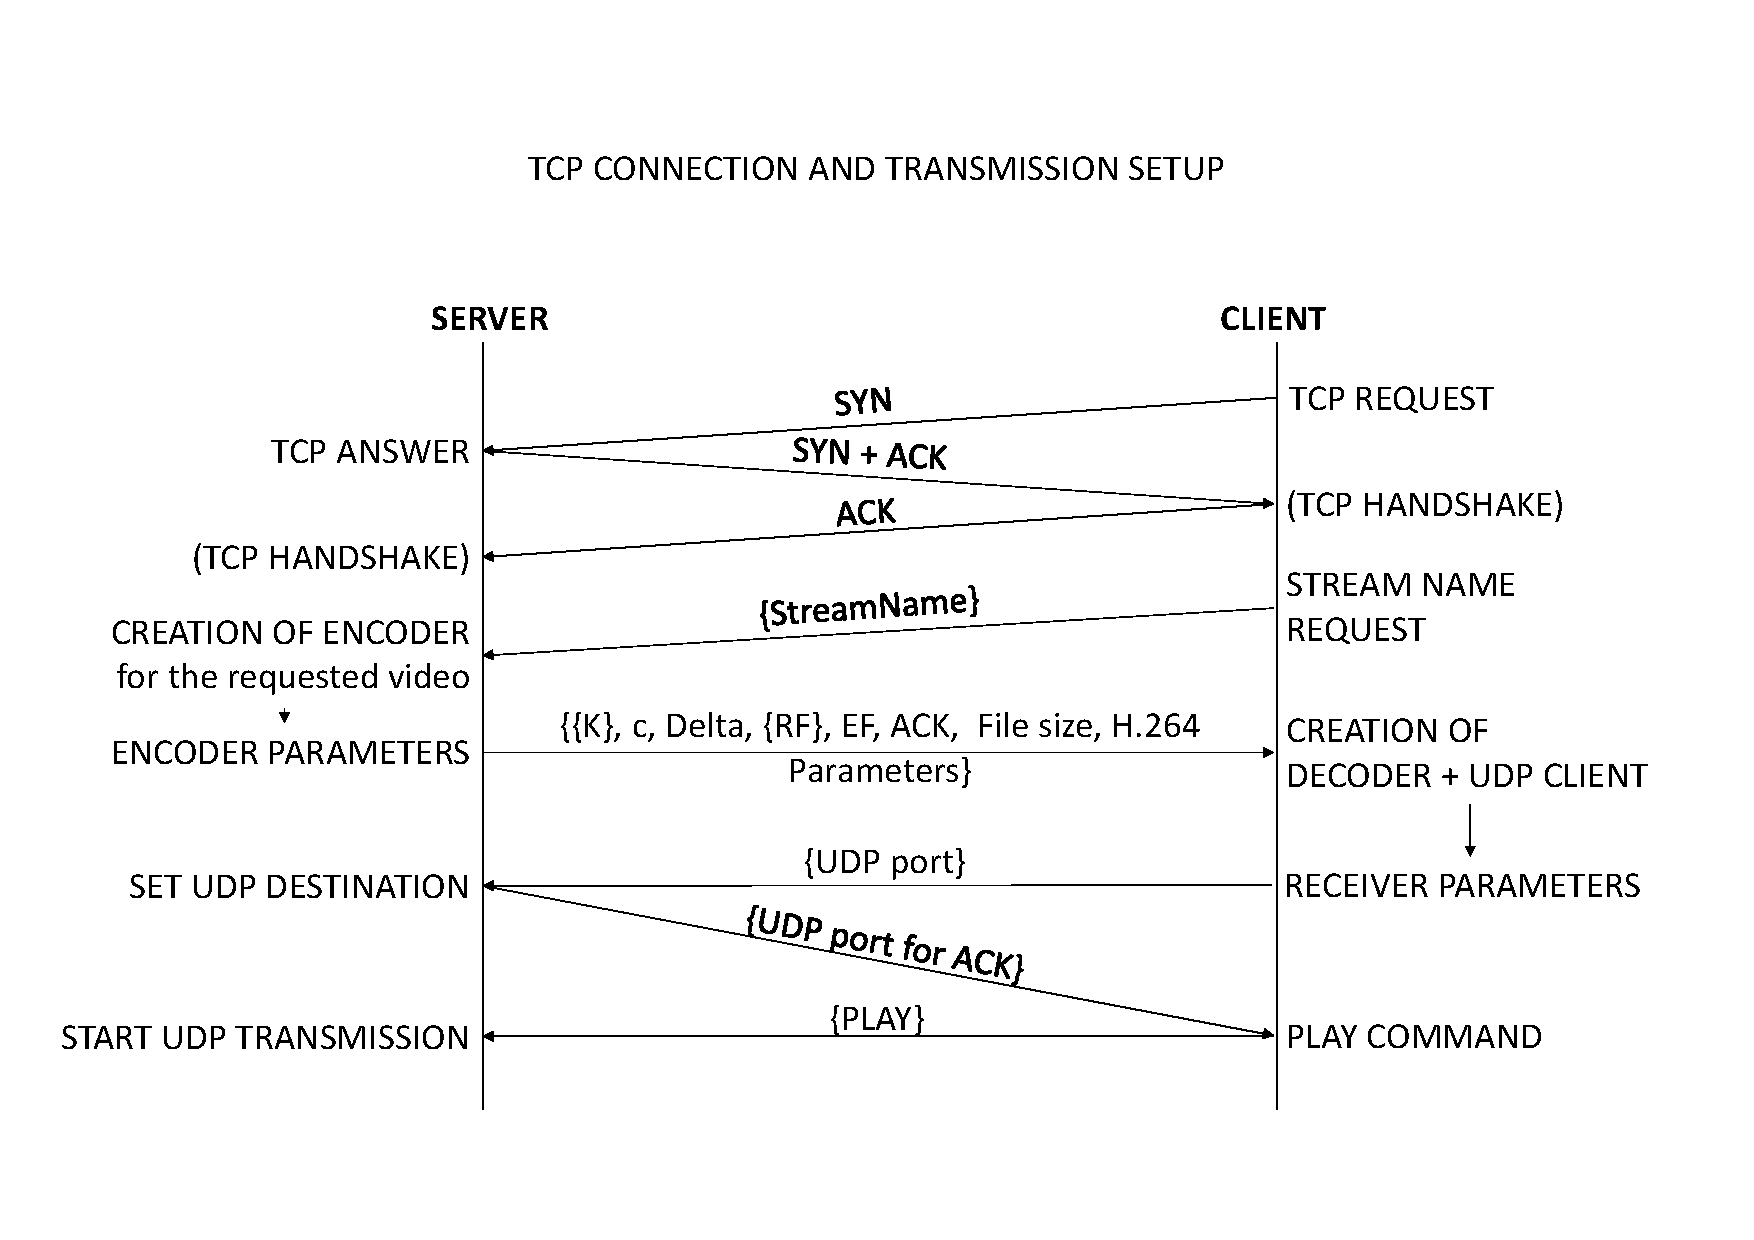
\includepdf{TCP.pdf}
\newpage
\subsection{Modelli matematici}
\subsubsection{Canale}
\label{sec:markov}
Il canale è rappresentato da una catena di Markov a 2 stati: buono (G) e cattivo (B).\\
Lo stato del sistema all'indice temporale $n$ (slot $n$) è indicato con $X(n)$, o $X_n$.\\
Sono stati effettuati test con due tipi di canale:
\begin{itemize}
\item Canale Markoviano, caratterizzato dalla seguente matrice di probabilità di transizione:\\
$$P=\begin{pmatrix}
P[X(n)=G, X(n+1)=G] & P[X(n)=G, X(n+1)=B]\\
P[X(n)=B, X(n+1)=G] & P[X(n)=B, X(n+1)=B]\\
\end{pmatrix} = \begin{pmatrix}
P_{GG} & P_{GB} \\
P_{BG} & P_{BB}
\end{pmatrix} =
\begin{pmatrix}
1-p & p \\
q & 1-q
\end{pmatrix}$$
Le probabilità stazionarie sono definite come
$$\bm{\pi} = \begin{pmatrix}
\pi_G\\\pi_B
\end{pmatrix} = \lim_{n \to\infty} \begin{pmatrix}
P[X(n)=G]\\
P[X(n)=B]
\end{pmatrix}$$
e possono essere ricavate dall'equazione
$$P^T\cdot \bm{\pi} = \bm{\pi} \Leftrightarrow \begin{pmatrix}
\pi_G\\
\pi_B
\end{pmatrix}=
\begin{pmatrix}
\frac{q}{p+q}\\
\frac{p}{p+q}
\end{pmatrix}$$
La probabilità stazionaria che il canale sia nello stato B è la probabilità d'errore media:
$$E[P_e] = \pi_B$$
Può essere definita la variabile aleatoria $\#_B$ che indica il numero di slot in cui il sistema resta nello stato B, la cui distribuzione di probabilità può essere scritta come:
$$P[\#_B=k]= \left(P_{BB}\right)^{k-1}P_{BG} = (1-q)^{k-1} q$$
Il valore atteso di $\#_B$ è l'inverso della probabilità di transizione da B a G:
$$E[\#_B] = \sum_{k=0}^{+\infty} k \cdot (1-q)^{k-1} q = q \cdot \frac{1}{(1-(1-q))^2} = \frac{1}{q}$$
I parametri impostati per il canale simulato sono stati il numero medio di slot B consecutivi, $E[\#_B]$, e la probabilità d'errore media $\pi_B$. In seguito sono state ricavate le seguenti quantità:
$$\begin{cases}q = \frac{1}{E[\#_B]}\\
\pi_G = 1- \pi_B\\
p = q\frac{\pi_B}{\pi_G}\end{cases}$$
\item Canale senza memoria, con packet error rate fisso $P_e$
\end{itemize}
Di seguito la rappresentazione Markoviana.
\begin{figure}[H]
    \centering
        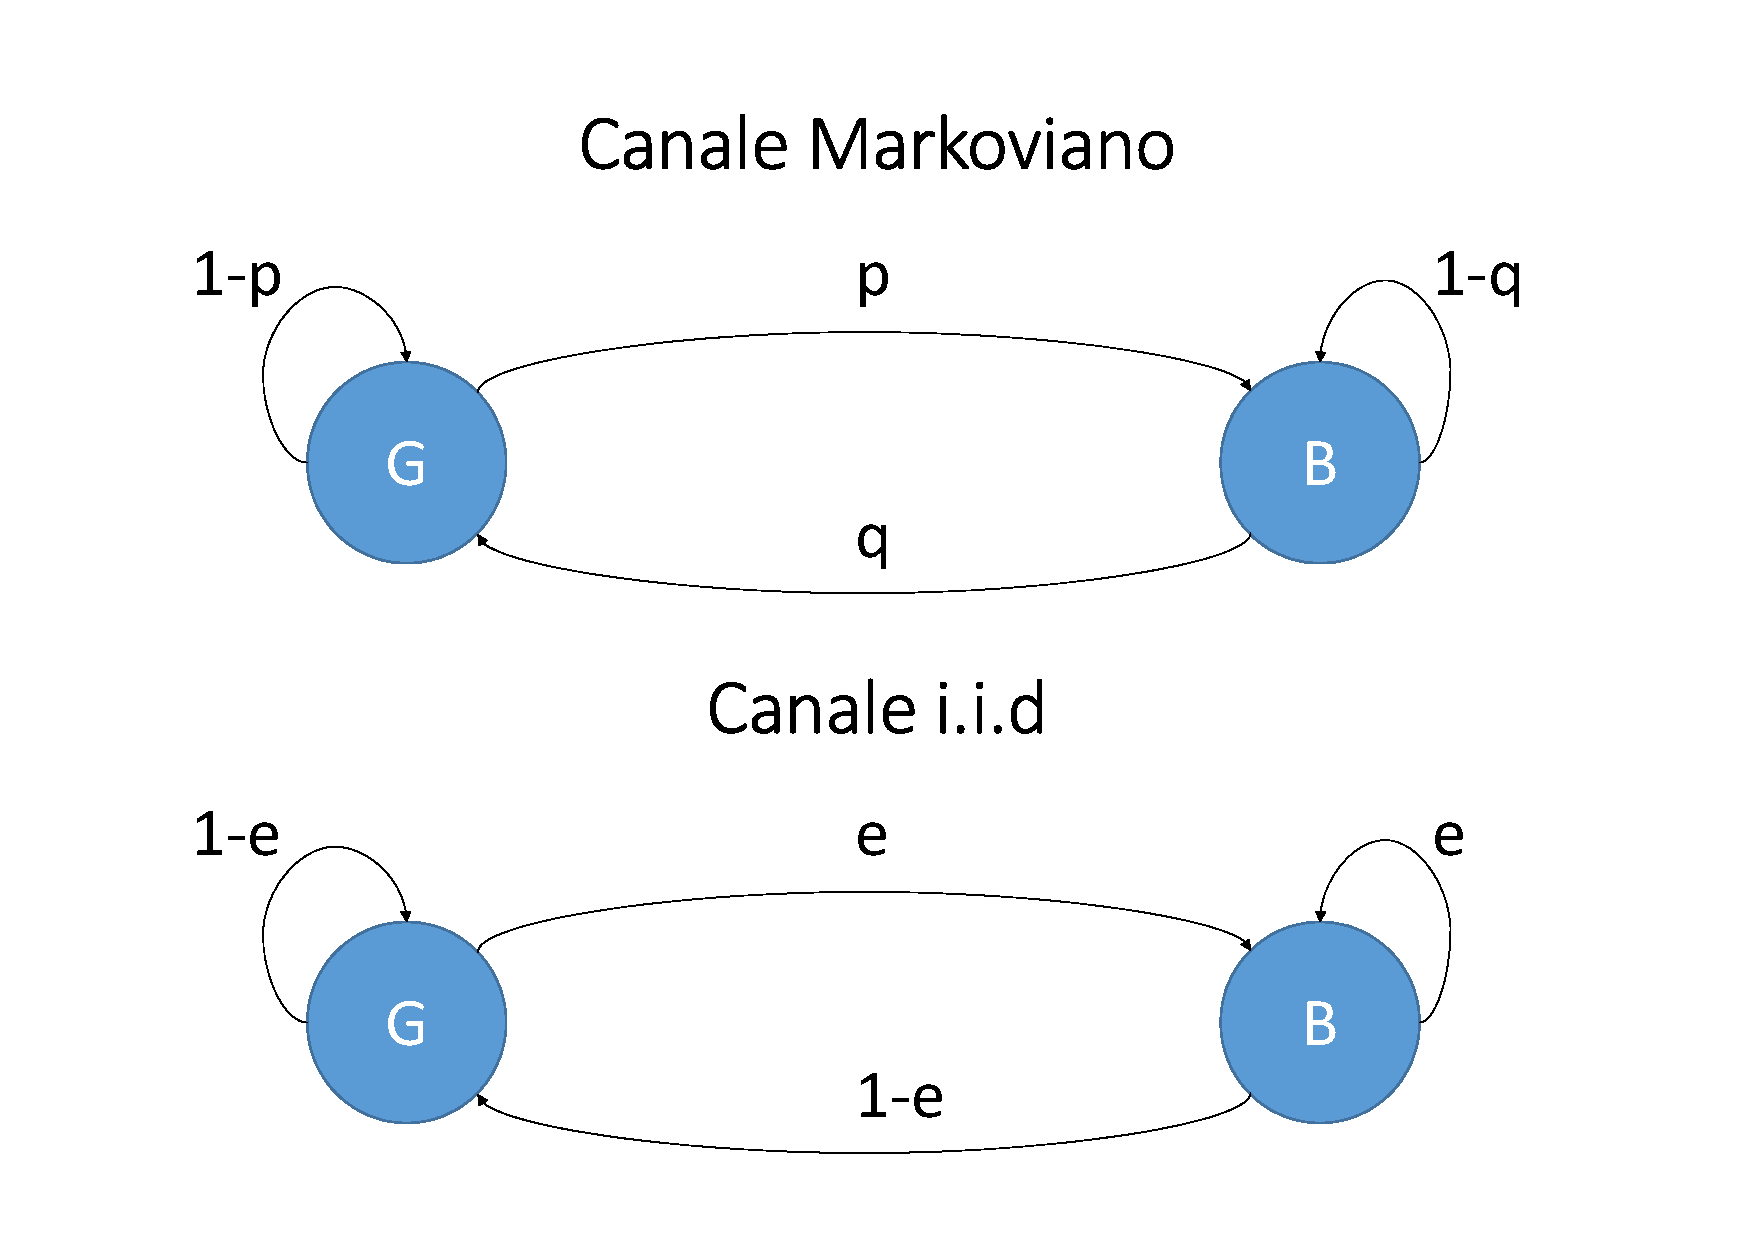
\includegraphics[clip, trim=0cm 1cm 0cm 1cm, width=0.5\textwidth]{Channel.pdf}
    \caption{Rappresentazione Markoviana dei due tipi di canale analizzati}
    \label{fig:Channel}
\end{figure}
\subsubsection{Codici a fontana}\label{FCsection}
I codici a fontana sono una classe di codici di correzione degli errori che aggiunge a un messaggio $\bm{x}\in\mathcal{A}^K$, di lunghezza $K$, una quantità di ridondanza potenzialmente infinita, aumentando la lunghezza del messaggio codificato $\bm{y}\in\mathcal{A}^N$, in modo tale che sia possibile recuperare il messaggio originale da un sottoinsieme di cardinalità leggermente maggiore di $K$ (e minore di $N$) del messaggio codificato.\\
%L'overhead introdotto dalla codifica è dato da $t = \frac{N-K}{K}$.\\
Fissando la lunghezza del messaggio codificato, $N$, per ogni messaggio originale di lunghezza $K<N$, è possibile schematizzare la codifica di canale lineare attraverso la seguente equazione
\begin{equation}
\bm{y} =
\begin{pmatrix}
y_1 \\y_2 \\y_3 \\\vdots \\y_N
\end{pmatrix} = \underbrace{\begin{pmatrix}
g_{11}	&g_{12}	&\cdots	&g_{1K}\\
g_{21}	&g_{22}	&\cdots	&g_{2K}\\
g_{31}	&g_{32}	&\cdots	&g_{3K}\\
\vdots &\ddots & \ddots &\vdots\\
g_{N1}	&g_{N2}	&\cdots	&g_{NK}
\end{pmatrix}}_{=G} \begin{pmatrix}
x_1 \\x_2 \\\vdots \\x_K
\end{pmatrix} = G \cdot \bm{x}
\end{equation}
dove $G$ è la matrice di codifica, $g_{ij}\in\{0,1\}$, $x_i\in\mathcal{X}$, $y_i\in\mathcal{Y}$.\\
La $i-$esima riga della matrice $G$ è casuale e il suo grado (la distanza di hamming dall'origine) segue una distribuzione di probailità nota: la Robust Soliton Distribution.\\
La codifica dell'$i-$esimo pacchetto avviene attraverso l'operazione di \textit{OR esclusivo} tra i pacchetti di informazione indicati dalla $i-$esima riga di $G$.\\
Se $G$ è invertibile, è possibile recuperare il vettore $\bm{x}$ da $\bm{y}$ attraverso la risoluzione di un sistema lineare.\\
I codici a fontana non prevedono la risoluzione di un sistema lineare per la decodifica, bensì un algoritmo di \textit{message passing}: con riferimento alla figura (\ref{fig:FC})
\begin{itemize}
        \item SE esiste un simbolo codificato $e_n$ con un solo arco entrante (come $e_4$)\begin{itemize}
                \item	Decodifica il simbolo di informazione corrispondente $i_k=e_n$ ($i_5$ in questo caso)
                \item	Rimpiazza tutti i simboli codificati $e_{n'}$ aventi un arco entrante da $i_k$ con $e_{n'}^{\text{new}} = e_{n'} \textit{ XOR } i_k$
                \item   Rimuovi gli archi da $i_k$
                \item   SE ci sono altri simboli di informazione da decodificare \begin{itemize}
                        \item Torna all'inizio
                \end{itemize}
                \item ALTRIMENTI\begin{itemize}
                        \item Decodifica riuscita
                \end{itemize}
        \end{itemize}

        \item ALTRIMENTI Decodifica fallita
\end{itemize}
\begin{figure}[H]
    \centering
        \makebox[\textwidth][c]{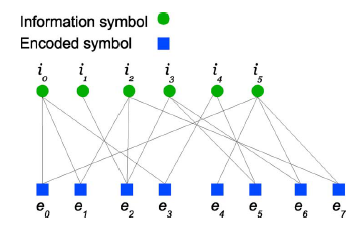
\includegraphics[width=6cm]{fc.png}}
    \caption{Schema: \textit{message passing}}
    \label{fig:FC}
\end{figure}
\newpage
\subsubsection{UEP}\label{UEPsection}
La protezione non uniforme di un messaggio prevede la divisione dello stesso in $p$ parti di diversa importanza.\\
Ogni parte viene ripetuta un numero $RF_i$ di volte, con $i\in\{1,\cdots,p\}$, in base alla sua importanza.\\
Il risultato della giustapposizione delle parti ripetute viene a sua volta ripetuto un numero $EF$ di volte.\\
Il messaggio che si ottiene da tali giustapposizioni è mappato nelle parti originali del messaggio originale e viene inviato al codificatore a fontana. Di seguito uno schema rappresentativo con $p=2$, $RF_1 = 2$,$RF_2=1$, $EF=2$.
\begin{figure}[H]
    \centering
        \makebox[\textwidth][c]{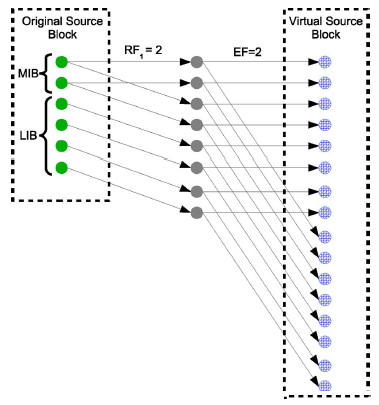
\includegraphics[width=8cm]{uep.png}}
    \caption{Schema della protezione non uniforme}
    \label{fig:UEP}
\end{figure}
\newpage
\section{Risultati}
L'algoritmo per la protezione non uniforme esposto nel
paragrafo~\ref{UEPsection} è stato testato nei due casi di canale senza
memoria e di canale Markoviano per determinare la packet error rate
ottenibile in queste due condizioni.

Sono stati inoltre misurati i tempi necessari alla codifica e
decodifica dei pacchetti in funzione dell'overhead desiderato.

Infine è stato misurato il PSNR ...

\subsection{Scelta della dimensione dei paccchetti}
Il paper \cite{uep} considera simboli di 1 byte durante la codifica,
ma questa scelta non è praticabile nel caso di questa tesina. Il
motivo è dato dall'overhead introdotto aggiungendo degli header a ogni
pacchetto, infatti una dimensione di pacchetto $L=1$ comporterebbe un
overhead del 1500 \% dovuto solo agli header.

Questo overhead decresce all'aumentare della dimensione dei pacchetti
$L$, tuttavia bisogna cohnsiderare l'overhead introdotto dalla
segmentazione del video H264.
%
Il video H264 è composto da pacchetti (detti NALU) di dimensioni
variabili che devono essere aggregati o segmentati in pacchetti di
dimensione fissa $L$. Il fatto di considerare due diverse classi di
priorità per le NALU richiede di inserire un certo numero di byte di
padding, ogni volta che termina una sequenza consecutiva di NALU con
la stessa priorità, per ottenere un numero intero di pacchetti di
lunghezza $L$.

Tenendo conto di entrambi questi contributi all'overhead si ottiene il
grafico mostrato in figura~\ref{fig:pktsize} ed è possibile
individuare il valore $L = 388$ che minimizza l'overhead dovuto al
padding e agli header.
% Best packet size = 388
% Min overhead = 0.069367
\begin{figure}[H]
  \centering
  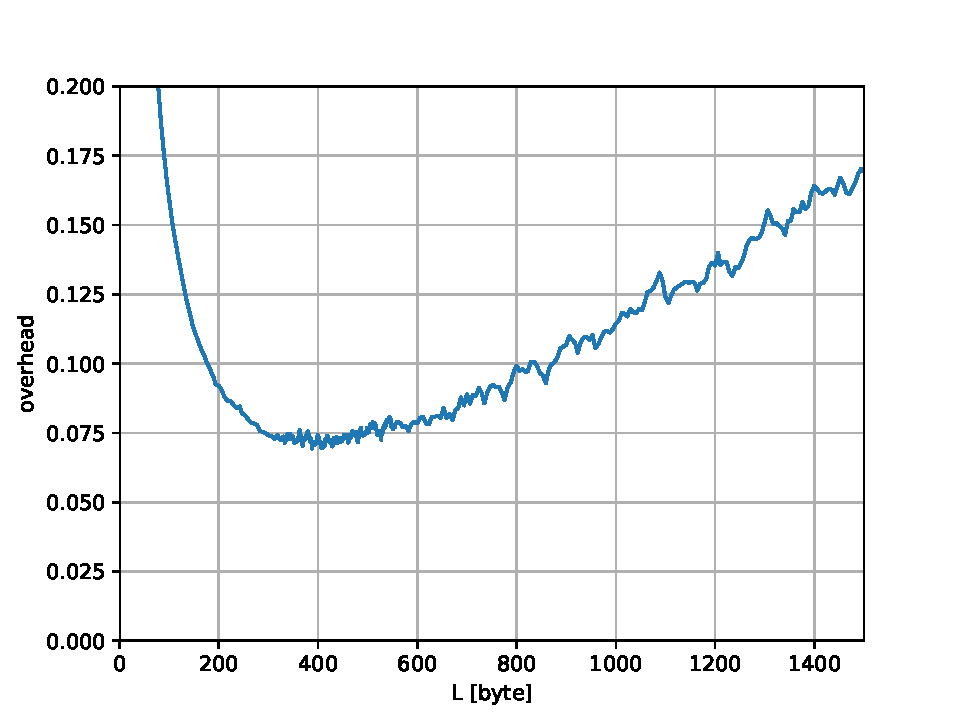
\includegraphics[width=0.8\textwidth]{plot_overhead}
  \caption{Overhead introdotto dalla segmentazione al variare della
    dimensione $L$ dei pacchetti.}
  \label{fig:pktsize}
\end{figure}

\subsection{Packet error rate su un canale senza memoria}
In questo caso è stata misurata la packet error rate a livello di
applicazione ottenuta variando l'overhead e considerando diversi
valori per la packet error rate del canale.
%
Facendo riferimento alla figura~\ref{fig:UDP}, la PER di livello
applicazione è misurata come la frazione di pacchetti forniti all'UEP
encoder che raggiungono l'uscita dell'UEP decoder.
%
L'overhead è definito, in modo analogo a \cite{uep}, come $t =
\frac{N-K}{K}$, cioè come l'aumento relativo del numero di pacchetti
trasmessi dovuto alla codifica.
%
Per permettere l'esecuzione di un gran numero di test, il server e il
client sono stati eseguiti sullo stesso computer, simulando un canale
senza memoria che scarta i pacchetti con una data probabilità $e$.

Sono stati usati gli stessi valori per i parametri specificati da
\cite{uep} per permettere un confronto con i risulati ottenuti in
questa tesina e di verificare la correttezza dell'implementazione.
%
I pacchetti in ingresso sono aggregati in blocchi di $K_0 = 100$
pacchetti importanti e $K_1 = 900$ pacchetti non importanti; il blocco
virtuale è stato costruito ripetendo $RF_0 = 3$ volte il primo
sotto-blocco, $RF_1 = 1$ il secondo ed espandendo la sequenza di
pacchetti così ottenuta di un fattore $EF = 4$. La lunghezza del
blocco virtuale è quindi pari a $EF \cdot \left( RF_0 \cdot K_0 + RF_1
\cdot K_1 \right) = 4800$ pacchetti.
%
L'overhead è stato fatto variare nell'intervallo $[0, 0.75]$, a cui
corrisponde un numero di pacchetti inviati $N \in [1000, 1750]$ per
ogni blocco di $K=K_0+K_1$ pacchetti.
%
La probabilità di errore del canale è stata impostata ai valori
$\left\{ 0, 10^{-2}, 10^{-1}, 3 \cdot 10^{-1} \right\}$.

Trasmettendo un video H264 segmentato in circa 400000 pacchetti,
ciascuno lungo 512 byte, attraverso il sistema UEP sono stati ottenuti
i risultati mostrati in figura~\ref{fig:iid}.
%
\begin{figure}[H]
    \centering
        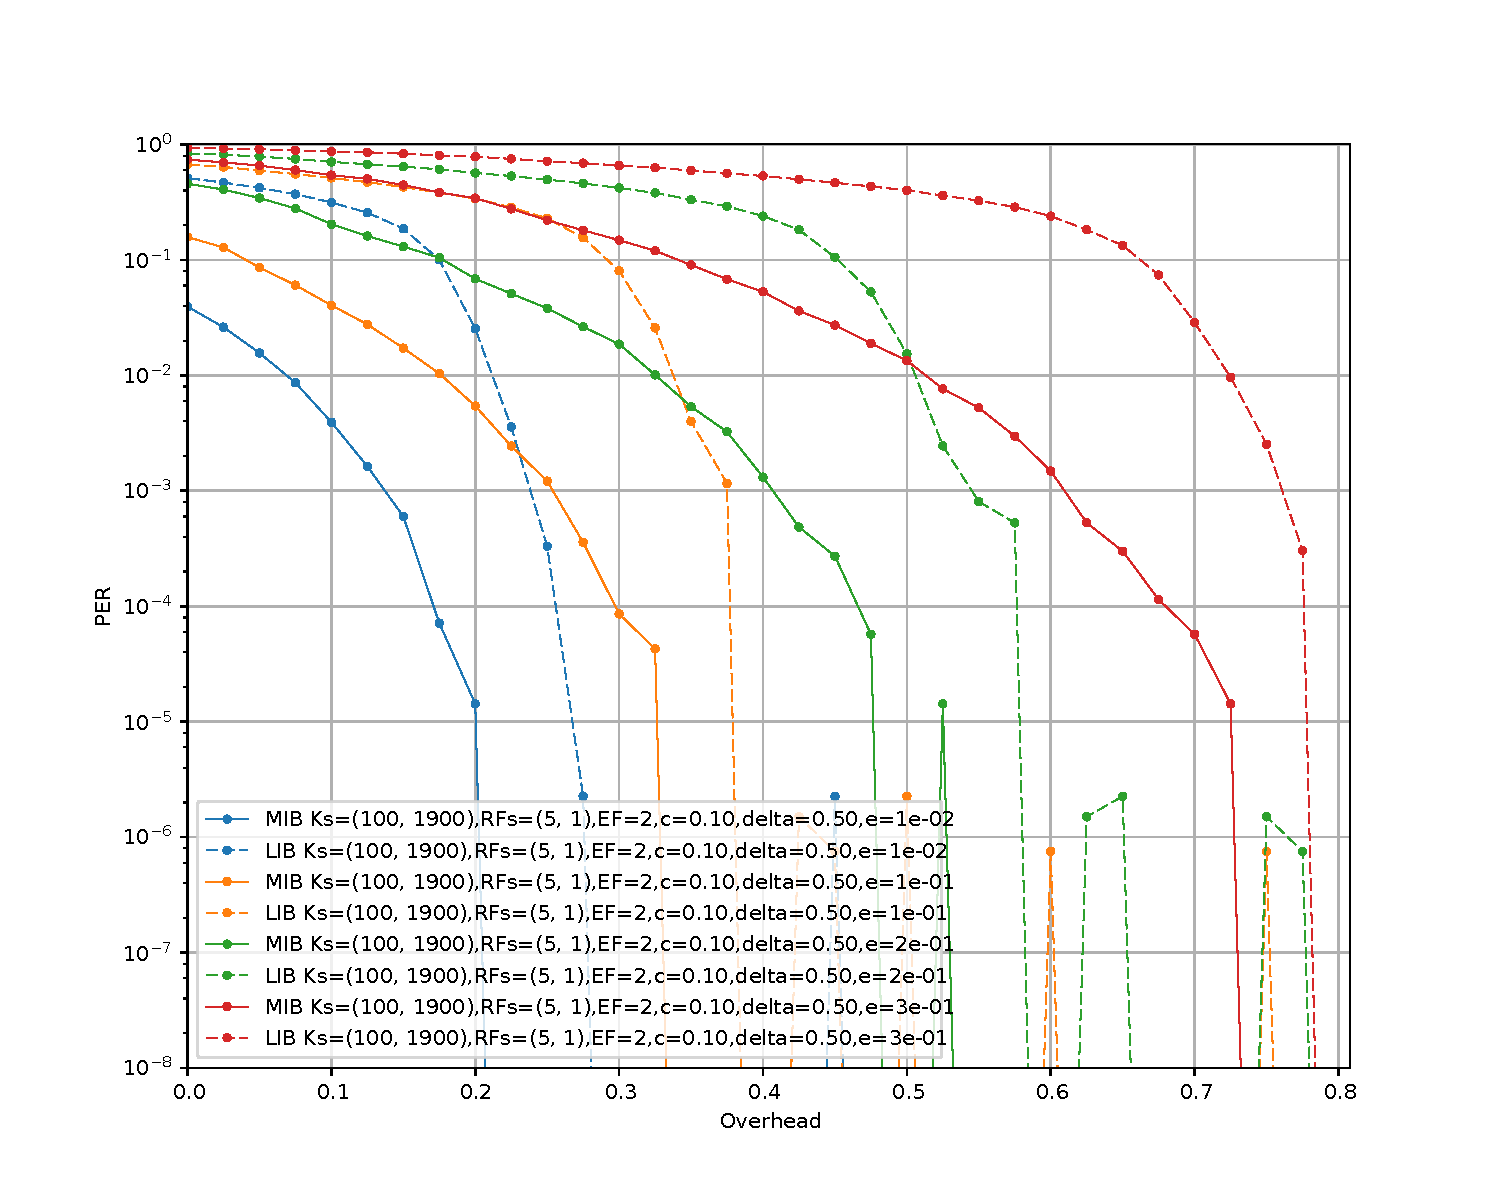
\includegraphics[clip, trim=0cm 0cm 0cm 0cm, width=0.80\textwidth]{plot_ber_iid.pdf}
    \caption{Packet error rate misurata su un canale iid al variare
    dell'overhead}
    \label{fig:iid}
\end{figure}
%
Come è possibile osservare, le curve corrispondenti al canale senza
errori ($e=0$) sono coerenti con \cite{uep}. Negli altri tre casi,
invece, la PER segue lo stesso andamento del caso senza errori ed è
semplicemente traslata verso destra di una lunghezza pari alla PER del
canale.
%
Si può infatti notare come nel caso $e = 10^{-2}$ l'algoritmo testato
abbia delle prestazioni molto vicine a quelle ottenibili su un canale
senza errori, mentre nei casi con PER $e = 10^{-1}$ ed $e = 3\cdot
10^{-1}$ le curve siano traslate, rispettivamente, di $0.1$ e $0.3$
rispetto al caso senza errori.

\subsection{Packet error rate su un canale Markoviano}
Nel caso del canale Markoviano, descritto nel
paragrafo~\ref{sec:markov}, sono state eseguite misure della packet
error rate variando la lunghezza media di una sequenza di slot cattivi
consecutivi e considerando diversi valori per la dimensione del blocco
$K$.
%
La frazione di pacchetti importanti presente in ogni blocco è stata
impostata al 10 \%, come per il caso iid, e anche per gli altri
parametri ($RF_i$ e $EF$) sono stati usati gli stessi valori dei test
precedenti.
%
\section{Conclusioni}


%\begin{figure}[H]
%	\makebox[\textwidth][c]{\includegraphics[width=16cm]{G10labE_f3.eps}}
%	\caption{Componenti di $\hat{s}$}\label{fig:s2}
%\end{figure}
\printbibliography[heading=bibnumbered, title=Bibliografia]
\end{document}
